\section{Beobachtungen} \label{chpt:Ergebnisse_Beobachtungen}
In diesem Kapitel werden umfassende Beobachtungen präsentiert, die eine detaillierte Bewertung der Leistung und Charakteristika des entwickelten Modells ermöglichen. Die Beobachtungen erstrecken sich über verschiedene Aspekte, einschließlich der Modellleistung nach dem Training, der Qualität der generierten Bilder sowie der Schnelligkeit und Qualität von Angriffen auf das Modell.
\subsection{Modellleistung}
Im Folgenden werden Metriken dargestellt und verglichen, mit Hilfe derer die Leistung der verschiedenen Modelle nach Abschluss der Trainingsroutinen bewertet werden kann.
\begin{figure}[H]
	\centering
	\begin{subfigure}[b]{0.35\linewidth}
		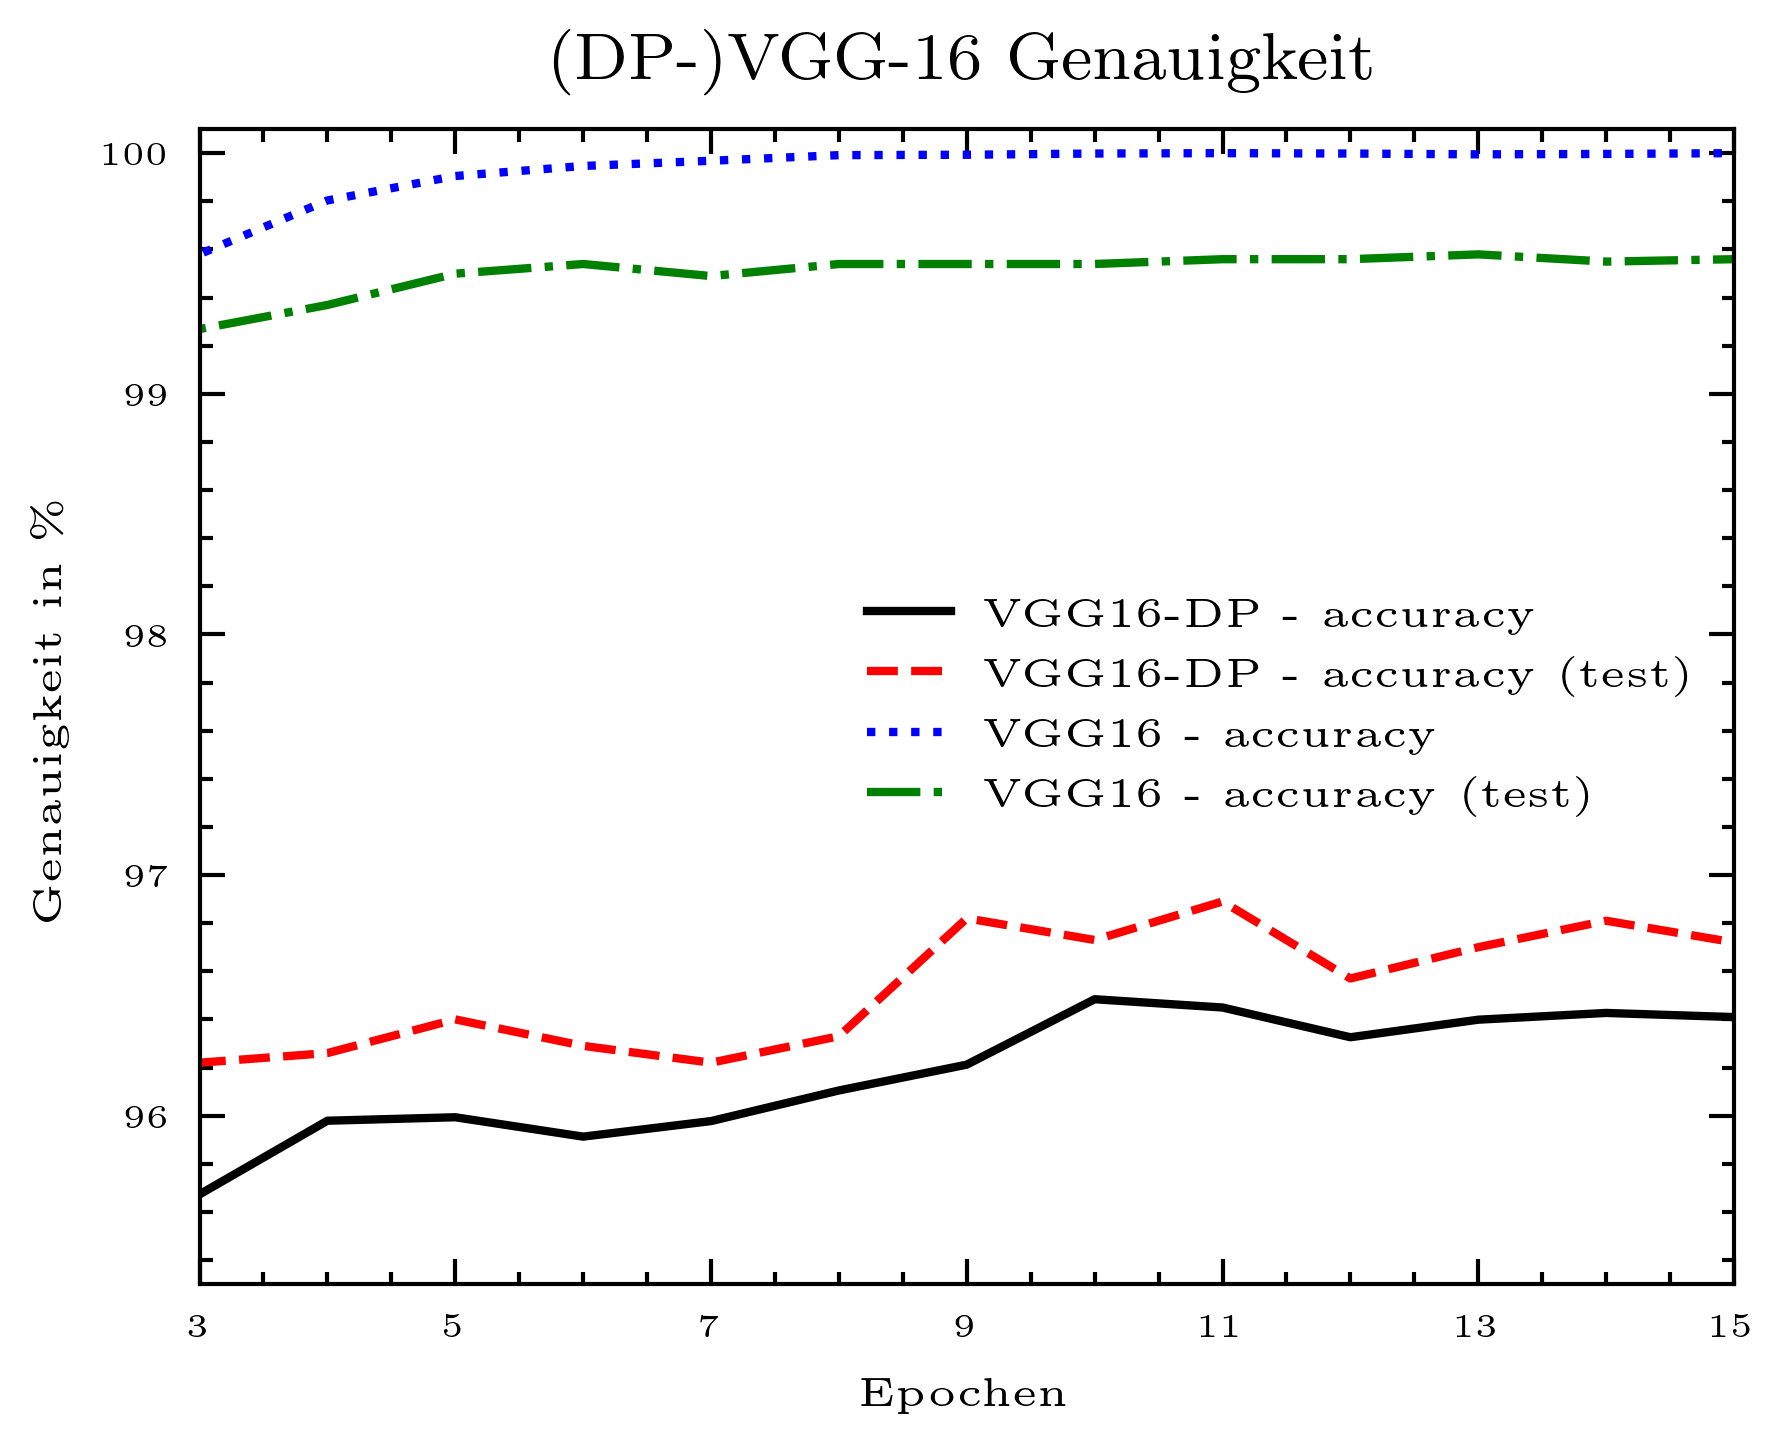
\includegraphics[width=\linewidth, height=4cm]{Bilder/acc.png}
		\caption{Modell-Genauigkeit}
		\label{img:acc_vgg_dp}
	\end{subfigure}
	\hspace{1cm} % Einfügen von horizontalen Abständen zwischen den Bildern
	\begin{subfigure}[b]{0.35\linewidth}
		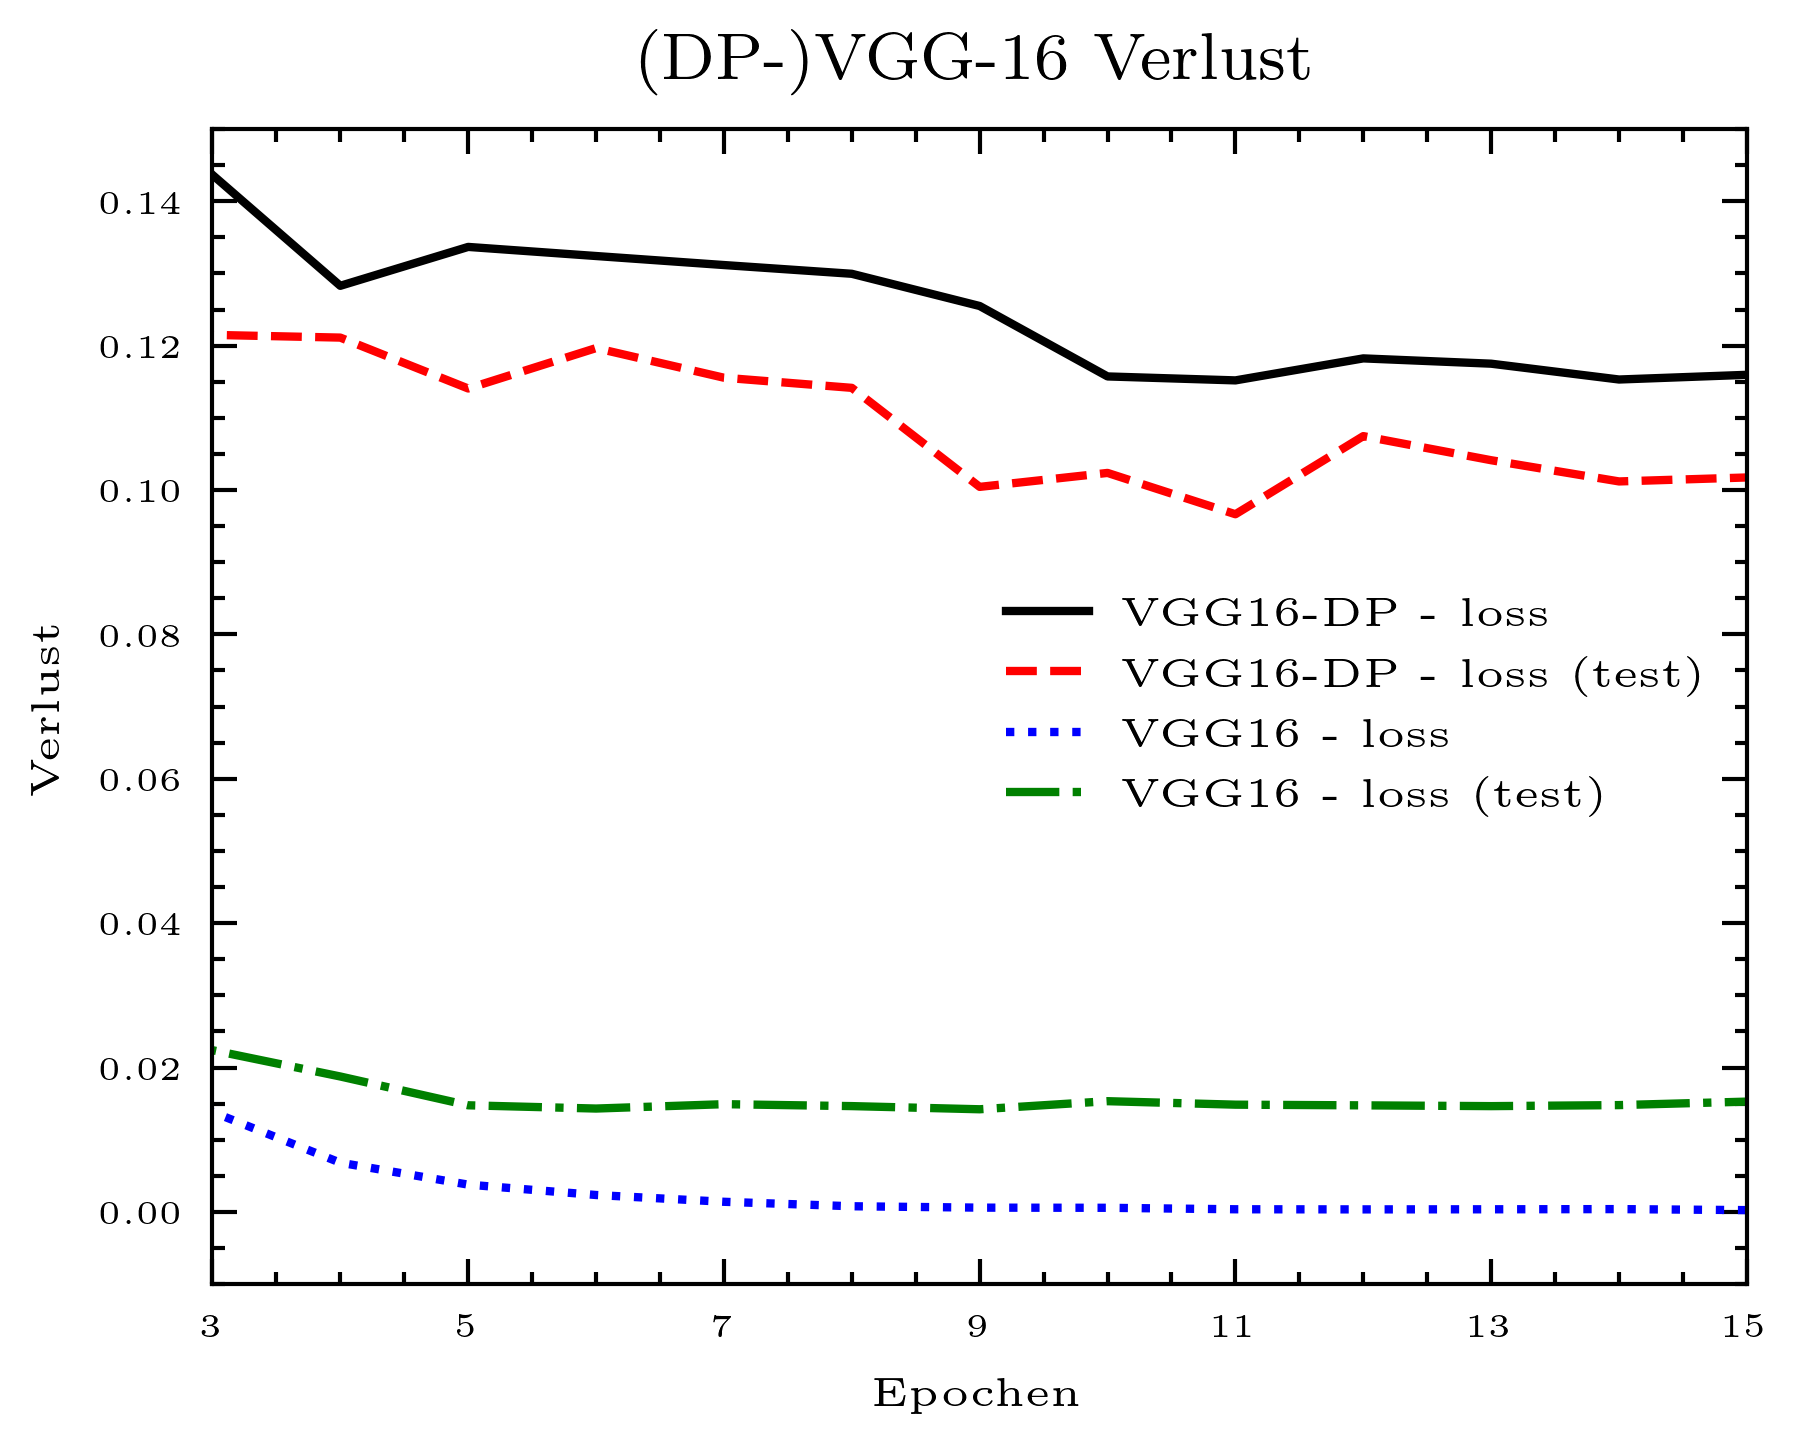
\includegraphics[width=\linewidth, height=4cm]{Bilder/loss.png}
		\caption{Verlust}
		\label{img:loss_vgg_dp}
	\end{subfigure}
	\caption{Verlust- und Genauigkeitsgegenüberstellung eines auf den MNIST-Datensatz normal und privat trainierten Modells}
	\label{img:mnist_figure}
\end{figure}
Die \textit{Genauigkeit} (Bild \ref{img:acc_vgg_dp}) bezüglich der Test- und Trainingsdaten nimmt -- wie erwartet -- im Laufe des Trainingsprozesses zu. Während das \glqq normale Training\grqq{} mit einer Test-Genauigkeit von $\approx99,0\%$ startet und bei $\approx 99,5\%$ nach etwa 7 Epochen stagniert, erreicht das \glqq neuronale Netzwerk mit differentieller Privatsphäre\grqq{} zu Beginn einen deutlich niedrigeren Wert von $\approx 91,5\%$ und stagniert während der trainierten 15 Epochen noch nicht. Dabei ist allerdings zu Vermuten, dass die Genauigkeit während weiteren Epochen ansteigt, was aufgrund begrenzter Ressourcen nicht getestet werden konnte. Die hohe Genauigkeit nach nur einer Trainingsepoche ist auf das Transfer-Learning zurückzuführen, wobei Gewichtungen des Modells schon anhand eines anderen, großen Datensatzes vortrainiert sind, und nicht mit Trainingsstart neu initialisiert werden müssen. 

Der \textit{Verlust} (Bild \ref{img:loss_vgg_dp}) während des Trainings zeigt einen ähnlichen Verlauf wie die oben beschriebene Test-Genauigkeit der beiden Modellarten. Nach etwa 7 Epochen beginnt dieser bei der Durchführung des \glqq normalen Trainings\grqq{} zu konvergieren und deutet darauf hin, dass das Training erfolgreich durchgeführt wurde. Im Gegensatz dazu ist wiederum bei dem \glqq Modell mit differentieller Privatsphäre\grqq{} zu beobachten, dass eine Konvergenz der Verlustfunktion nach 15 Epochen nicht erkannt werden kann. Auch hier -- wie bei Test-Genauigkeit -- lässt sich vermuten, dass eine Erhöhung der Trainingsdurchläufe eine Minimierung der Verlust-Funktion herbeiführt.  Zudem lässt sich bei beiden Modellen aus dem Verlauf der Verlustfunktion ableiten, dass die Modelle keine Überanpassung bezügliche der Trainingsdaten vorweisen. 

Das \glqq normale Training\grqq{} kann aufgrund der konvergierenden Verlust- und Genauigkeitsverte nach 7 Epochen beendet werden, da die Parameter nahezu vollständig an den Datensatz (Bild \ref{img:mnist_figure} - MNIST) angepasst sind. Dahingegen sollte man aufgrund der unvollständigen Parameteranpassung im Modell mit differentieller Privatsphäre die Anzahl der Epochen  erhöhen.

\subsection{Bildqualität}
Aufgrund der verschiedenen Angriffs-Verfahren variiert die Genauigkeit der Bilder in den unterschiedlichen Durchgängen, wobei die Qualität - abhängig von der Komplexität des Generative-Adversarial Networks - gleich ist. Die Genauigkeit des neu generierten Bildes, das aus privaten Daten abgeleitet ist, wird mit Hilfe des Confidence-Scores bezüglich Ziel-Klasse bestimmt. Im Folgenden werden einige Vergleiche über die Bildqualität nach der Ausführung des Angriffs basierend auf einem Klassifizierungsmodell für Zahlen und Gesichtern aufgezeigt.

Die \textit{Qualität} der Bilder ist abhängig von genutztem GAN (Generative adversarial network), das für die Generierung verwendet wird. Generierungen basierend auf dem DCGAN sind aufgrund geringerer Parameter, kürzerer Trainingsdauer und anderer Faktoren qualitativ nicht so hochwertig wie die des genutzten StyleGANs.

\begin{figure}[H]
	\centering
	\begin{subfigure}[b]{0.35\linewidth}
		
\includegraphics[width=\linewidth]{Bilder/0_mnist.png}
		\caption{Generierung der Zahl 0 auf Basis eines DCGAN}
		\label{img:gen_img_dcgan}
	\end{subfigure}
	\hspace{1cm} % Einfügen von horizontalen Abständen zwischen den Bildern
	\begin{subfigure}[b]{0.35\linewidth}
		
\includegraphics[width=\linewidth]{Bilder/401_celeba.png}
		\caption{Generierung einer Frau mit Hilfe eines StyleGANs}
		\label{img:gen_img_stylegan}
	\end{subfigure}
	\caption{Bildqualität der GAN-Modelle}
	\label{img:gen_img}
\end{figure}
Die Bilder des DCGAN basierten Generators sind etwas schwach mit vergleichsweise wenigen Pixeln aufgelöst (siehe Bild \ref{img:gen_img_dcgan}). Dahingegen lassen sich Bilder des StyleGAN Netzwerks in einer deutlich besseren Auflösung von bis zu 200 $\times$ 200 Pixeln generiern. Wie im Bild \ref{img:gen_img_stylegan} zu erkennen, wird die Qualität der Bilder durch die Reduktion der Pixel deutlich verschlechtert, was aber zu einer effektiveren Angriffsdauer führt. Im Gegensatz zu den generierten Ziffern handelt es sich bei den Gesichtern um 3-Kanal Bilder (RGB), weshalb diese farblich zu betrachtet sind.
\subsection{Angriffsperformance}
Dieses Kapitel befasst sich mit der Auswertung beider Angriffe nach der Durchführung, wobei im Folgenden ein Vergleich mit dem Ziel der Stärken- und Schwächenbeleuchtung aufgestellt wird. Um die Angriffe besser bewerten zu können, werden zum einen visuelle, aber auch metrische Daten begutachtet, wozu beispielsweise die Genauigkeit der neu generierten Bilder bezüglich der Ziel-Kategorie des \glqq angegriffenen\grqq{} Modells zählt.
\subsubsection{Bildqualität der Angriffe}
\subsubsection{Angriffsstatistiken}
% Genauigkeit normal
% Dauer
\subsection{Auswertung der Verteidigungsstrategie}
% Genauigkeit dp